\documentclass[conference, letterpaper]{IEEEtran}
%\documentclass[a4paper]{article}

\ifCLASSINFOpdf \else \fi

\usepackage[pass]{geometry} \usepackage{tabularx} \usepackage{graphicx}
\usepackage{amssymb} \usepackage{algorithm} \usepackage{algorithmic}
\usepackage{amsmath} \usepackage{booktabs} \usepackage{caption}

\usepackage{cite} \usepackage[numbers,sort&compress]{natbib}
\captionsetup[table]{position=top,labelfont={sc},textfont={sl}}

\renewcommand{\thetable}{\Roman {table}}

\title{ Use of Model Predictive Control (MPC) for Rocket Altitude Correction }

\author{ \IEEEauthorblockN{Nikhil Peri, Anthony Lin, Manit Ginoya, Paul Buzuloiu } \
\IEEEauthorblockA{uOttawa Rocketry Team \\ \{nperi104, alin102
mgino015, pbuzu025\}@uottawa.ca} }

\begin{document}
\maketitle
\begin{abstract}
\end{abstract}

Keywords—Model Predictive Control, Aerospace.  \section{Introduction}

Rockets unlike other aircraft have high speed and dynamic flights, as a result
rocket control systems have to be extremely responsive and precise. Classical
control systems based on observed sensor feedback would not be able to meet the
demands of rocket flight since the latency between plant actuation affecting the
the physical world and detecting that change through sensor observations is too
slow for such dynamic flight enviroments. Model Predictive Control (MPC) solves
these problems by introducing state estimation.  This process involves maintianing
a kenetic

\section{Airbrake Model}

\section{Model Predictive Control}

The complexity of rocket flight partially arises from the numerous states
required to fully define an entire set of dynamics. These states include
acceleration, velocity, position, orientation, angular speed and angular
acceleration of the rocket in all three spatial dimensions. Additionally,
the states related to the actuators (in this case, the servo motor controlling
the airbrakes) must also be considered. Desiging a classical controller or even
a digitally implmented classicial controller would bring along several
inconveniences; for this reason, a model predictive controller was considered
and implemented.

The major concept of model predictive control is to maintain a real time
simulation; This simulation's role is to produce a prediction of future system
states using feedback from sensors and the system's current states. For the case
of achiving a particular target altitude by deploying airbrakes, the MPC will
produce a predicted final altitude
every control loop. Using this predicted final altitude, the error between the
predicted final altitude and the desired final altitude will be calculated. The
final part of the MPC process is to map the calculated error to a specific
(whether heuristic or deterministic) control signal that will be sent to the
airbrake actuator.

Figure \ref{fig:MPC_diagram} is the fully defined control system diagram
corresponding to the description provided above. Running through the control
schema yeilds the following sequence of events: sensors are read, filtered and
fused, states are estimated, trajectory is predicted, final altitude error is
determined, control signal is generated, signal is sent to actuator driver,
actuation occurs which affects rocket flight.

\begin{figure}[H]
\centering
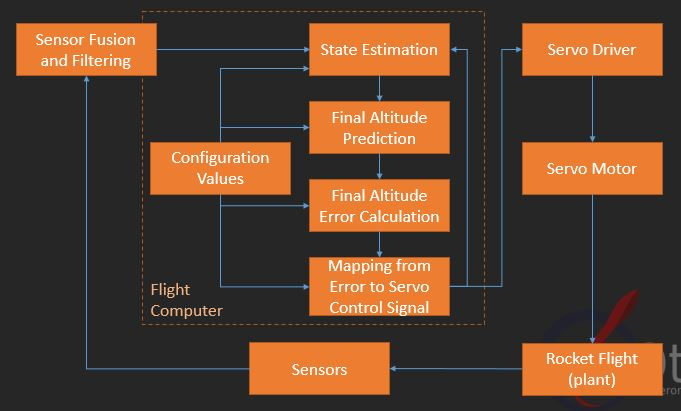
\includegraphics[width=0.45\textwidth]{./MPC_diagram}
\caption{Overall Control Diagram of airbrake system}
\label{fig:MPC_diagram}
\end{figure}

When comparing figure \ref{fig:MPC_diagram} to a
typical control systems diagram, the input to the system seems to be missing;
This input (the desired final altitude) is merely hidden away as a part of the
digitally implemented configuration values. Some important inferences of the
presented control diagram include understanding that the configuration values
include all phycial rocket parameters, as well as the desired final altitude.
Therefore, the presented figure is related more to the physcial implementation
than to control theory notation.

\section{Imeplementation}



\section{Conclusion}

\section{Acknowledgement}

\bibliographystyle{unsrt}
\bibliography{references}
\end{document}
